%********VORAUSSETZUNGEN & GRUNDLAGEN*********
\chapter{Fundumentals}
\label{sec:Fundumentals}
\section{Scanning Tunneling Microscopy (STM) }
The Scanning Tunneling Microscope was introduced in 1981 by Gerd Binning and Heinrich Roherer. 
With this measuring technique it is possible to resolve a conductive surface with a precission far beyond that of conventional light based Microscopes.
In contrast to other electron based microscopy like Scanning Electron Microscopes (SEM), it uses the quantum mechanical phenomenon of tunneling.
In classical mechanics, objects cannot overcome a potential barrier if their energy E is smaller than the barrier $E < V_0$, as observed in gravitational interactions.
This phenomenon observed for quantum mechanical particles like electrons, which can surpass a potential barrier despite the initial expectation for classical mechanics that they should not be able to.
The STM uses this effect by precisely positioning a sharp conductive tip close to the surface and applying a bias voltage.
The distance between the tip and  the sample then represents the tunneling barrier.
By varying the bias voltage, the tunneling probability can be changed, thereby affecting the tunneling current.
If the bias voltage, also referred to as the potential difference, is kept constant, the tunneling current is primarily dependent on the distance between tip and surface.
Thus the tip-sample distance can be acurately measured in the sub \AA ngström range by measuring the tunneling current.
The tip is moved in the x-,y-plane, where a grid is established, measuring the tip-sample distance for each grid point, a topographic image of the sample surface can be created. 
There are two modes of operation, the constant-height mode, where the tip is held at a constant height above the sample while scanning and the change in tunneling current is measured, and the constant-current mode, where the tip height is adjusted to keep the tunneling current constant during scanning.

\newpage
\begin{wrapfigure}{r}{0.5\textwidth}
    \centering
    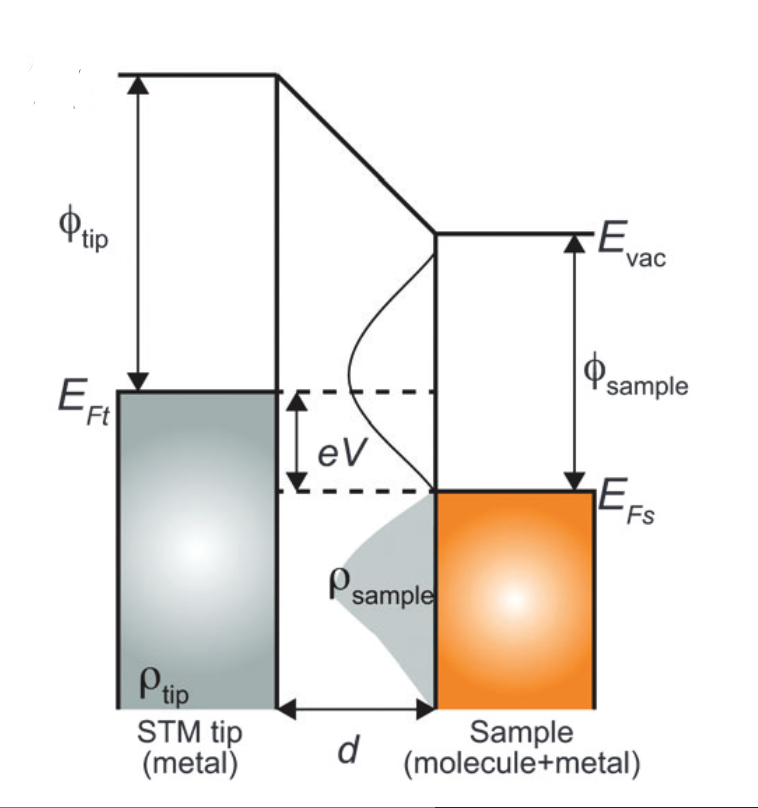
\includegraphics[width=0.4\textwidth]{graphics/Tunneling_diagram_japan.PNG}
    \caption{Energy diagram of the tunneling  junction with a positive bias voltage applied. $\Phi_{tip}$ \& $\Phi_{sample}$: work functions of tip and sample, $E_{vac}$: vacuum energy level,  $E_{ft}$ \& $E_{fs}$: Fermi Energys of the tip and sample,  $\rho_{tip}$ \& $\rho_{sample}$: density of states of tip and sample,  $eV$: potential difference caused by applying a bias Voltage $V$ (picture source: \cite{Kano}) }
    \label{fig:energy_diagram}
\end{wrapfigure}

The tunneling current,is not only influenced by the sample geometry/topography , but also by the electronic structure of tip and sample.
If the tip is in the vicinity of the metallic substrate the fermi energies align, resulting in an equal probability of electrons tunneling from the tip to the sample and vice versa.
This consequently results in a zero net current. 
Through the introduction of a bias voltage $U_{bias}$ the fermi energies of tip and sample can be shifted relative to each other (Figure \ref{fig:energy_diagram}).
If the bias voltage is positive, the fermi energy of the sample is pushed down and electrons from occupied states in the tip can tunnel into the empty states of the sample.
Consequently if the bias voltage is negative, electrons from the filled states of the sample tunnel into the tip.
The tunneling current is influenced by the distance $d$ between orbitals of the tip and the sample, which makes it possible to gain information about the electronic structure of the sample.
This is not really a representation of the real structure of the atoms or molecules, but the electronic Local Density of States (LDOS) of the sample´s surface.
Utilizing this in Scanning Tunneling Spectroscopy (STS) provides additional information beyond the sample's topography, such as the chemical composition, bonding, the energy gap and band-bending effects. \cite{cbai}
\newpage
\subsection{Theoretical Foundations of STM}

A detailed description of the tip-sample interaction is provided by the model developed by Tersoff and Hamann. \cite{PhysRevLett}
Here, the tip is approximated as spherical potential well (Figure \ref{fig:tip_scheme}). $R$ is in that case the radius of the tip located at position $\vec{r_0}$ with the distance $d$ from the surface.
First order pertubation theory then gives the following expression (Eq. \ref{eq:tunneling_pert}) for the tunneling current of this system :
\begin{equation}
    I = \frac{2 \pi e}{\hbar} \sum_{\mu \nu} f(E_{\mu})[1 - f(E_{\nu}+eV_{bias})]\cdot |M_{\mu \nu}|^2 \delta(E_{\mu}- E_{\nu})
    \label{eq:tunneling_pert}
\end{equation}\\

\begin{wrapfigure}{r}{0.3\textwidth}
    \centering
    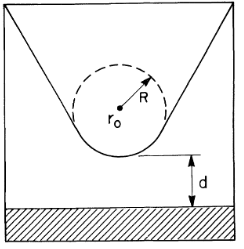
\includegraphics[width=0.3\textwidth]{graphics/fundamental_tip_sheme.PNG}
    \caption{Schematic depiction of the tip geometry \cite{PhysRevLett}}
    \label{fig:tip_scheme}
\end{wrapfigure}

\noindent The fermi distribution $f(E)= (\exp((E-E_F)/k_b T)+1)^{-1}$ gives the ocupation probability of a fermion (electrons) with the Energy $E$ near the fermi level.
In this case it is the occupation probability of the tip states (denoted by the subindex $\mu$) and the occupation probability of the sample states (denoted by the subindex $\nu$).
The tunneling matrix $M_{\mu \nu}$ is related to the derivatives of the sample wave functions $\psi_{\nu} $ at the nucleus of the apex atom \cite{tunnelmatrix}.
When STM Imaging is done at low temperatures and with small voltages, Equation \ref{eq:tunneling_pert} can be simplified to:
\begin{equation}
    I = \frac{2 \pi}{\hbar} e^2 V_{bias} \sum_{\mu \nu}  |M_{\mu \nu}|^2 \delta(E{\nu}-E_F) \delta(E_{\mu}- E_{F})
    \label{eq:tunneling_pert_simple}
\end{equation}
With the tunneling matrix $M_{\mu \nu}$ , which relates to the probability of an electron transitioning from state $\mu$ to state $\nu$ \cite{tunnelmatrix}.
It is defined as the surface integral over the seperation surface $\Sigma$, where $d\vec{S}$ is the surface element on $\Sigma$.: 
\begin{equation}
    M_{\mu \nu} = \frac{\hbar^2}{2m} \int_{\Sigma} (\psi_{\mu}^{*} \vec{\nabla} \psi_{\nu} - \psi_{\nu} \vec{\nabla} \psi_{\mu}^{*}) \, d\vec{S}
    \label{eq:tunnelin_matrix}
\end{equation}
To obtain a solution, the tip wave function can be explicitly chosen as an s-type orbital, which reduces complexity through the introduction of symmetry.
This orbital has a spherical form \cite{PhysRevLett}:
\begin{equation}
    \psi_{\mu} = \Omega_t^{-1/2} * c_t k R e^{kR} ( k|\vec{r}- \vec{r_0}|)^{-1} e^{-k|\vec{r}- \vec{r_0}|}
    \label{eq:tip_wave}
\end{equation}
$\Omega_t^{-1/2}$ is the volume of the probe, $k = \hbar^{-1} \sqrt{2m\phi}$ is the inverse dacay length for the wave functions in vacuum, $c_t$ is a geometry specific constant on the order of 1 and $R$ is the radius of curvuture.
The surface wavefunctions can be approximated as blochwaves, which are plane waves modulated by a periodic function.
In the region of neglible Potential the surface wavefunction can be written as:
\begin{equation}
    \psi_{\nu} = \Omega_{s}^{-1/2} \sum_{G} a_G \exp(- (k^2 + |\vec{k}_{||} + \vec{G}|^2)^{1/2} z)\cdot \exp(i(\vec{k}_{||} + \vec{G})\cdot \vec{x})
    \label{eq:surface_wave}
\end{equation}
Here $\Omega_{s}^{-1/2}$ is the sample volume, $k$ the previously mentioned inverse decay length, $\vec{k}_{||}$ is the surface bloch wave vector and $\vec{G}$ represents the reciprocal surface vector.
Substituting into \ref{eq:tunneling_pert_simple} gives the result:
\begin{equation}
    I = 32 \pi^3e^2 V_{bias}\phi^2 D_t(E_F)R^2 k^{-4} e^{2kR} \cdot \sum_{\nu} |\psi_{\nu}(\vec{r_0})|^2 \delta(E_{\nu} - E_F) 
\end{equation}
Where $D_t(E_F)$ is the Density of States of the Tip at the Fermi Level. 
The sum over the local states of the surface $\psi_{\nu}$ at the Fermi Level ($\delta(E_{\nu} - E_F)$) can be interpreted as the Local Density of States (LDOS).
Using the surface wavefunction one can see that the tunneling current decreases exponentially with increasing tip sample distance $d$.
Because of this exponential dependence, the tip height can be measured with such high precision. :
\begin{equation}
    I \varpropto e^{-2 \cdot d \sqrt{\frac{2m \phi}{\hbar^2}}}
    \label{eq:propcurrent}
\end{equation}




\newpage

\section{Low Energy Electrons Diffraction (LEED)}
\noindent LEED is a simple technique that can image periodic structures present at the sample surface.
A collimated beam of electrons with the same wavelengh is directed at a flat surface.
In this case the wavelengh of the incoming electrons is determened by the electric field $U_a$ that accelerates them (see Eq.\ref{eq:electron_wavelengh}).
To see diffraction the wavelengh of the electrons must be in the range of the lattice constant.
The kinetic energy of the electrons is up to $E_{kin} = e U_a = 200$ eV.
\begin{equation}
    \lambda = \frac{h}{\sqrt{2 m_e e U_a}}
    \label{eq:electron_wavelengh}
\end{equation} 
If a periodic structure is present at the surface, a sharp pattern of spots can be observed, which corresponds to the k-space of this structure.
\begin{wrapfigure}{r}{0.6\textwidth}
    \centering
    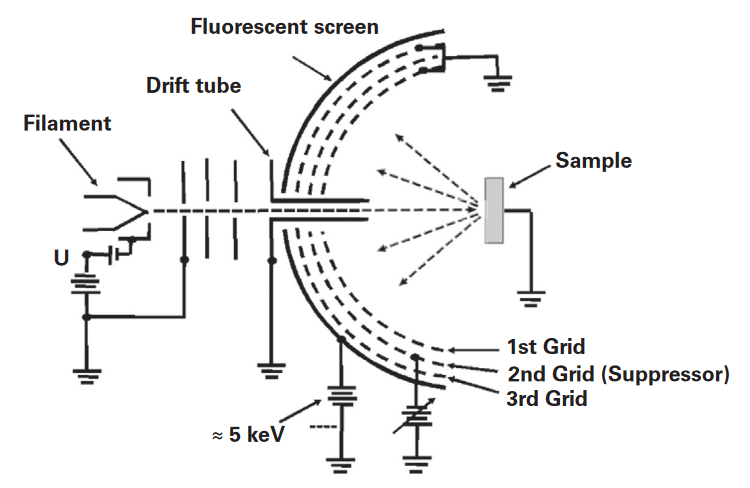
\includegraphics[width=0.5\textwidth]{graphics/fundamental_leed_setup.PNG}
    \caption{A basic three-grid LEED system which utilizes a flourenscent screen as imaging tool \cite{MoritzWolfgang2022SSDb}}
    \label{fig:LEED_Shematics}
\end{wrapfigure}
\noindent The LEED setup consists of a filament which emitts electrons by applying a current.
These electrons are then accelerated and collimated in a drift tube which points at the sample.
Due to interactions of the electrons with the crystal atoms some of them are not diffracted elastically.
To ensure that only the elastically scattered electrons are show on the flourencent screen, a grid system is installed in front of the screen.
The first grid and the sample are both grounded to ensure that the diffracted electrons propagate undisturbed through the space between the sample and the grid.
A filter Voltage is aplied between the second and third grid that is just below the acceleration voltage.
Electrons which are not elastically scattered are completely stopped, which makes it effectivelly a high pass filter. \cite{MoritzWolfgang2022SSDb} \\
The collimated beam can be represented as a planar wave $e^{i \vec{k_0} \vec{r}}$  outside the surface.
The wavevector $\vec{k_0}$ points in the propagation direction and represents the spacial frequency of the wave.
This vector can be modeled as:
\begin{align}
    |\vec{k_0}| &= \frac{2 \pi}{\lambda} = \frac{\sqrt{2 m_e E}}{\hbar} \\
    \hspace{1cm} \notag \\
    \vec{k_0} &= \begin{pmatrix}
        |k_0|\cos(\varphi)\sin(\vartheta)\\|k_0|\sin(\vartheta)\sin(\vartheta)\\|k_0| \cos(\vartheta)
    \end{pmatrix}
\end{align}
A 2D periodic surface structure with a reciprocal basis ($b_1$,$b_2$) causes the plane waves to diffract.
The diffracted waves are described as $A_g e^{i \vec{k_g} \vec{r}}$ with wave vectors $|\vec{k_g}| = |\vec{k_0}|$.
$\vec{k_g}$ transforms according to $\vec{k_g} = \vec{k_0} + \vec{g}$.
The reciprocal lattice vector $\vec{g} = 2 \pi ( h b_1 + k b_2)$ represents the individual points where constructive interference is present.
Usually the indices h and k are intergers which characterize the beam, for example (0,0) or (1,1).
It can be shown that the wave vector in vacuum outside the surface is \cite{MoritzWolfgang2022SSDb}:
\begin{equation}
    k_g = - \sqrt{\frac{2 m_e E}{\hbar^2} - (k_{0x}+ g_{x})^2 - (k_{0y}+ g_{y})^2}
\end{equation}

%\polyfig{graphics/fundamental_kspace.PNG}{hllohi}{fig:kspace}{graphics/fundamental_kspace_theta.PNG}{fig:kspace_}{helo}

%\begin{figure}[H]
%    \centering
%    \begin{minipage}[b]{0.49\textwidth}
%        \centering
%        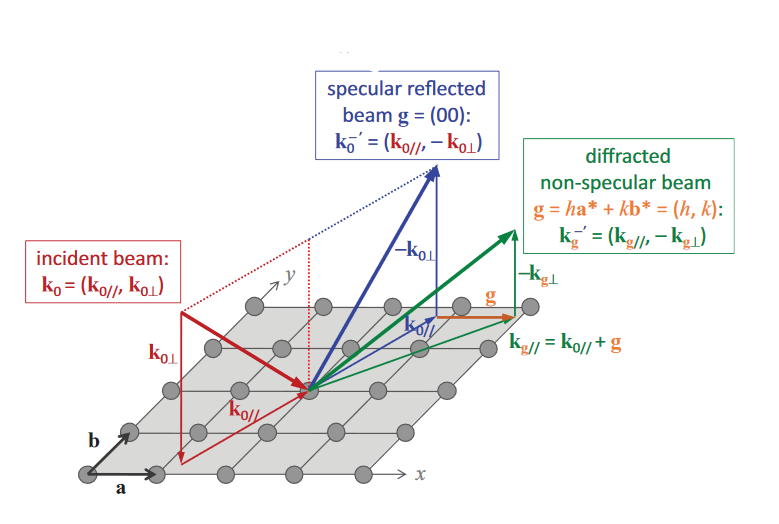
\includegraphics[width=\textwidth]{graphics/fundamental_kspace.PNG}
%        \caption{
%            2D lattice with the reciprocal lattice vectors $\vec{a}$ and $\vec{b}$. 
%            $\vec{k_0}$ (red): incident beam,
%            $\vec{k_{0}^{-}}'$ (blue): specular reflected beam,
%            $\vec{k_{g}^{-}}'$ (green): non-specular diffracted beam, }
%        \label{fig:kspace}
%    \end{minipage}
%    \begin{minipage}[b]{0.49\textwidth}
%        \centering
%        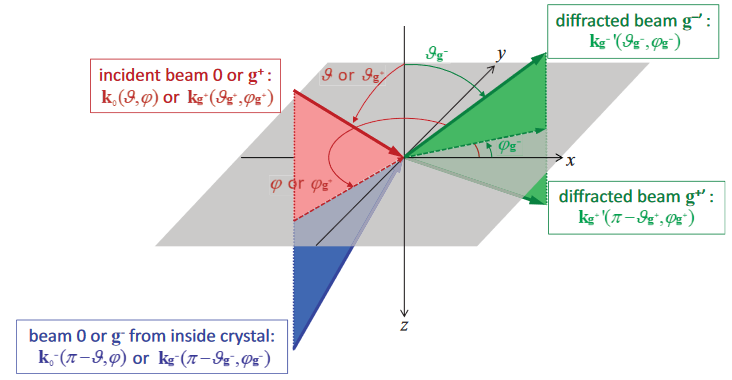
\includegraphics[width=\textwidth]{graphics/fundamental_kspace_theta.PNG}
%        
%        \caption{hgh}
%        \label{fig:kspace2}
%    \end{minipage}
%\end{figure}
%
\monofig{width=0.7\textwidth}{graphics/fundamental_kspace.PNG}{2D lattice with the reciprocal lattice vectors $\vec{a}$ and $\vec{b}$. 
$\vec{k_0}$ (red): incident beam,
$\vec{k_{0}^{-}}'$ (blue): specular reflected beam,
$\vec{k_{g}^{-}}'$ (green): non-specular diffracted beam,
$\vec{g}$ (orange): 2-D reciprocal lattice vector <hk>. \cite{MoritzWolfgang2022SSDb}}{fig:kspace}

%\duofigcom{graphics/fundamental_kspace.PNG}{fig:kspace}{graphics/fundamental_kspace_theta.PNG}{fig:kspace2}{
%    (a): 2D lattice with the reciprocal lattice vectors $\vec{a}$ and $\vec{b}$. 
%    $\vec{k_0}$ (red): incident beam,
%    $\vec{k_{0}^{-}}'$ (blue): specular reflected beam,
%    $\vec{k_{g}^{-}}'$ (green): non-specular diffracted beam, }{}
%

\newpage


\section{Energy Alignment}
This section was heavily influenced by and based on the research presented in the PhD thesis of Michael Hollerer, titled "Charge Transfer through thin
Dielectric Films: Organic Molecules
on MgO(001)/Ag(001)". \cite{hollerercharge}
The concept of energy level alignment is crucial for the understanding of adsorption of organic molecules on inorganic substrates like Ag or MgO.
It can result in altered properties of molecules and can influence their electronic structure.
Therefore it is subject of ongoing research. \cite{braun2009energy}
As it is important for the explanation of some observed effects in the obtained experimental data a brief summary is provided.\\
\begin{wrapfigure}{r}{0.6\textwidth}
    \centering
    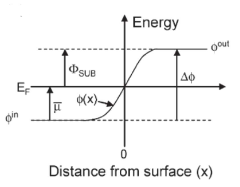
\includegraphics[width=0.5\textwidth]{graphics/workfunction.PNG}
    \caption{The substrate workfunction  $\phi_{SUB}$ consisting of the bulk chemical potential $\bar{\mu}$ and the electric dipole $\Delta \phi$. \cite{hollerercharge}}
    \label{fig:workwork}
\end{wrapfigure}
\noindent The energy needed for extraction of an electron from a solid to a point in the vacuum far from the surface is defined as the workfunction. 
It is defined as the sum of the bulk chemical potential $\mu$ and the electrostatic surface dipole $\Delta \phi$.
\begin{equation}
    \Phi = - \mu + \Delta \phi
\end{equation}
In metals the electrostatic potential arises from electron spill-out which creates a dipole at the surface.
While the local workfunction can vary depending on the local structure, it is averaged at further distances which gives rise to the global workfunction.
For single crystal metals this energy can vary depending on the crystal plane exposed to the vacuum, and is mostly influenced by how closely packed it is.
Mathematically, it can be expressed as the difference between the vacuum energy level and the Fermi energy:

\begin{equation}
    \phi = E_{Vac} - E_F
\end{equation}
This even holds true for insulators like like MgO and other oxides with a large band gap.
In metals the density of states is continuous around the fermi energy, which makes electronic states available for conduction.
The occupation of states around $E_F$ follows the Fermi-Dirac-Distribution and is influenced by the temperature.
Organic Molecules on the other hand have discrete energy levels for orbitals, with the most important for adsorption being the Highest Occupied Molecular Orbital (HOMO) and the Lowest Unoccupied Molecular Orbital (LUMO).
The energy gained by bringing an electron from the vacuum energy level to the LUMO energy level is called the Electron Affinity (EA), while the energy needed to bring an electron from the HOMO to the vacuum level is called the Ionisation Energy (IE).
When a molecule is adsorbed onto the surface the vacuum levels of the substrate and the molecule align.
If the substrate has a high workfunction and the molecules Electron Affinity is smaller, the molecule will most likely adsorb in a neutral charge state.
If on the other hand the molecules EA is high enough, or the substrate work function low enough, the LUMO is pushed under the Fermi-Energy Level, which means that charge transfer into the LUMO will occur.
This is due to the fact that all states below $E_F$ are occupied.\\
%\textbf{Energy Alignment Mechanisms}\\
%\duofigcom{graphics/Energy Alignment/energyalignmetal.PNG}{fig:metalad}{graphics/Energy Alignment/energyaligndielectric.PNG}{fig:dielectricad}{}{}
\monofig{width=0.7\textwidth}{graphics/Energy Alignment/energyalignmetal.PNG}{Energy Level Alignment process of an organic molecule (Pentacene) adsorbed onto a metal substrate.  \cite{hollerercharge}}{fig:en_al_ag}
\monofig{width=0.7\textwidth}{graphics/Energy Alignment/energyaligndielectric.PNG}{Energy Level Alignment process of an organic molecule (Pentacene) adsorbed onto a dielectric/metal substrate. Note that the push-back effect arises from the dielectric/metal interaction.\cite{hollerercharge}}{fig:en_al_mgo}
% EA: Electron Affinity of the Molecule, IE: Ionization Energy of the molecule,$\phi_{metal}$: the metals workfunction, $\Delta \phi_{CT}$: workfunction change induced by charge transfer. ,$\phi_{Final}$: Final workfunction after adsorbtion 
\subsection{Push-Back}
As discussed earlier, a non-zero negative charge is observed outside the surface. 
This is commonly known as the electron spill-out and results in an electric dipole, which in turn contributes to the work function of the substrate. 
Upon adsorption of the molecule, the electronic states interact, leading to Pauli Repulsion. 
This, in turn, pushes the charge back into the surface and reduces the electric dipole, consequently reducing the work function in respect to the Fermi Energy.
\subsection{Polarization}
The surface charges rearrange upon adsorbtion of a polarizable molecule, which intern manifests in an attractive interaction with unoccupied states and an repulsive interaction with occupied states.
This results in a decrease of the LUMO-HOMO gap in respect to the gas-phase LUMO-HOMO gap of the adsorbates.
In this process the workfunction of the substrate does not change, because no overall dipole perpendicular to the surface is introduced.

\subsection{Charge-Transfer (CT)}
If the LUMO is shifted below the Fermi Energy ($E_F$) of the metal substrate, it becomes (partially) occupied.
This is due to the fact that metals have a continuous density of states at $E_F$ with no bandgap.
The molecules frontier orbitals therefore hybridize with the metal states resulting in an overlap of the molecular wavefunctions with a corresponding substrate state. 
This results in partial occupation of the LUMO, which is referred to as Fractional Charge Transfer (FCT) \cite{savu2015fingerprint}.
If looking at thin dielectric films on metal substrates like MgO on Ag, no FCT is observed.
In contrast to metals, dielectric materials do not have continuous DoS at the Fermi Level and therefore no states available for hybridization. 
For a low initial workfunction and a high EA like depicted in Fig \ref{fig:en_al_mgo} the LUMO is pushed below $E_F$.
As a consequence of this, electrons will tunnel through the dielectric layer to occupy it.
Electrons can only tunnel as a whole, and therefore it is referred to as "Integer Charge Transfer (ICT)".
This leads to the formation of a surface dipole, which in turn increases the workfunction.
It should be noted that the charge transfer from the molecule to the substrate is also possible if the IE is low and the initial workfunction is high.
This workfunction increase then raises the LUMO energy, CT continues either until all available LUMOs are occupied, or the LUMO has been raised in energy up to $E_F$, at which point CT stops.
This process is called Fermi-level pinning and will play a significant role in the explanation of observed phenomena in this thesis.








\newpage